\section{Part 1}
\subsection*{Binary Density Estimation}
Modeling $\Pr(x=1)$ given IID samples $x^1,x^2,\dots,x^n$.
\subsection*{Bernoulli Parameterization}
Bernoulli Distribution over binary variable, parametrized by $\theta$.
\[\Pr(x\mid\theta)=\theta^x (1-\theta)^{1-x}\]
\subsection*{Binary Inference Tasks}
\begin{enumerate}
    \item Computing Probabilities
    \item Computing Dataset Probabilities
    \item Decoding
    \item Decoding Dataset
    \item Sampling
\end{enumerate}
\subsection*{Why sample?}
\begin{enumerate}
    \item Model Interpretation
    \item Approximate Quantities
    \item Interested in Samples, etc.
\end{enumerate}
\subsection*{Learning Strategies}
See Learning Principles.
\[\theta_{MLE} = \frac{n_1}{n}\]
\subsection*{Beta distribution (prior)}
\[\Pr(\theta\mid\alpha,\beta)\propto \theta^{\alpha-1}(1-\theta)^{\beta-1}\]
\[\alpha=\beta=1\Rightarrow MLE\]
\[\alpha=\beta=2\Rightarrow \text{Laplace Smoothing}\]
Laplace Smoothing adds extra imaginary '1' and '0'.
\subsection*{Multivariate Binary Density Estimation}
Inference tasks, joint, marginal, conditional prob
\begin{enumerate}
    \item Computing Joint Probabilities $\Pr(x_1,\dots,x_d)$
    \item Computing Marginal Probabilities $\Pr(x_1)$
    \item Computing Conditional Probabilities $\Pr(x_1\mid x_2)$
    \item Decoding Dataset
    \item Sampling
\end{enumerate}
Product of Bernoullis assumes variables independent.
\subsection*{Generative Classifiers}
Model joint prob, $\Pr(x,y)$\\
Naive Bayes uses product of Bernoullis for $\Pr(x\mid y)$.
\subsection*{Discriminative Classifiers}
Model $\Pr(y\mid x)$\\
Tabular parameterization - fit parameter for $\Pr(y=1\mid x)$ for each $x$.\\
\subsection*{Logistic Regression}
$\Pr(y\mid x)$ using sigmoid function.\\
MLE is convex optimization, gradient descent.
\subsection*{Sigmoid/$\tanh$}
\[S(x)=\frac{1}{1+e^{-x}}\in(0,1)\]
\[\tanh(x)=\frac{e^x-e^{-x}}{e^x+e^{-x}}\in(-1,1)\]
\subsection*{Fundamental Trade-Off}
Simple models no overfit may underfit, complicated models vice versa.
\subsection*{Neural Networks}
One Layer
\[\tilde{y}=\sum_{c=1}^k v_c h(w_c^T x_i + b_c) + \beta\]
Learns features and classifier simultaneously\\
Universal Approximator if layer grows w $n$ examples\\
Non-Convex problem, SGD works, implicit regularization\\
\subsection*{Deep Learning}
\[\tilde{y}=v^T h(W^4 h(W^3 h(W^2 h(W^1 x))))\]
Vanishing gradient problem - away from origin, gradient nearly 0\\
ReLU, skip connections, ResNets\\
NN Heuristics
\subsection*{Double Descent Curves}
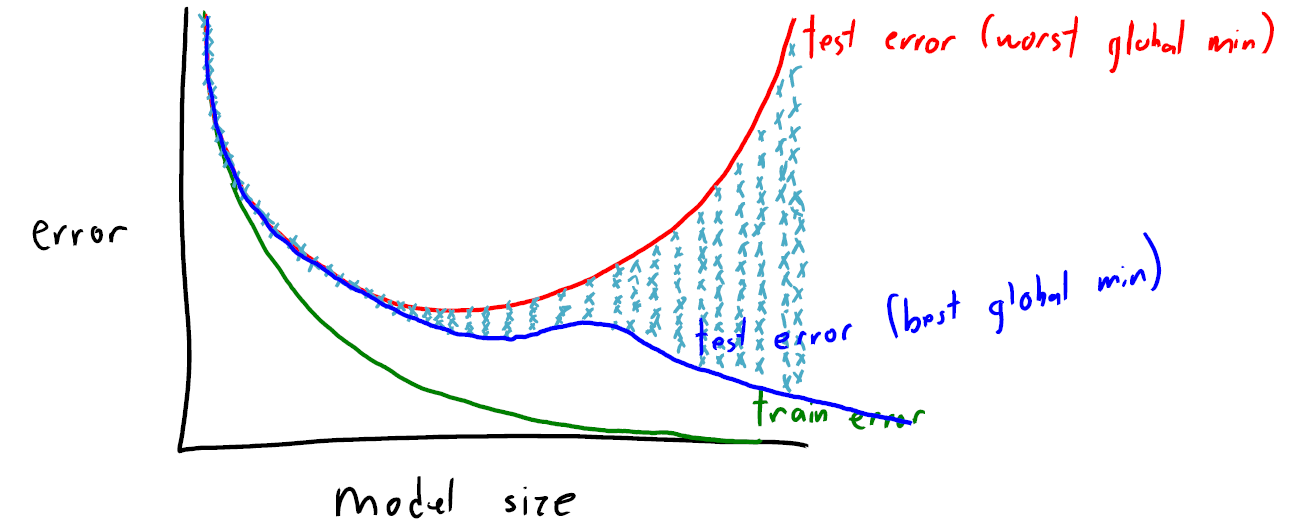
\includegraphics[width=\linewidth]{contents/dd.png}
From A2, alternatively increase regularization strength as you add features
\subsection*{ResNets}
\[a^{l+2}=h(a^l+W^{l+1}h(W^l a^l))\]
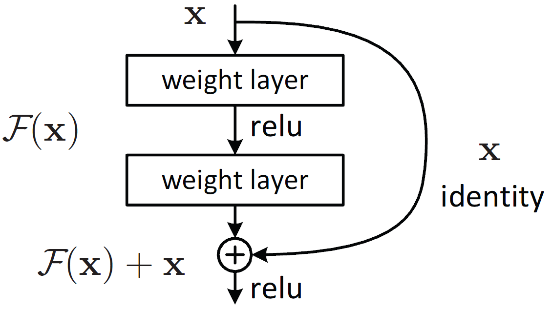
\includegraphics[width=\linewidth]{contents/resnet.png}
\subsection*{Automatic Differentiation}
Code generates gradient code (chain rule)\\
Advantage - get gradient for same cost as function\\
Disadvantage - Store all intermediate calculations, same cost as computing function (may have lower cost to calculate gradient for some functions)
\subsection*{CNN}
Convolutions transfrm images, can approximate directional derivatives and integrals at different scales.\\
Convolution layers, max pooling layers, reduces no. of params, gives spatial invariance
\subsection*{Autoencoders}
Output is input
Encodes input into bottleneck layer, then decodes back to input\\
Bottleneck forces compression, cannot just memorize\\
Non-linear dimensionality reduction\\
Denoising Autoencoders learn to enhance images
\subsection*{Multi-Label Classification}
0-k correct labels\\
Encoding-Decoding approach: classes shares hidden layers, reduce params, model dependencies
\subsection*{Pixel Labeling}
Fully Convolutional networks maintain spatial information at all layers\\
Upsampling for pixel Classification
